\input ../SlidePreamble
\input ../preamble

\newcommand{\solution}[1]{\bigskip {\bf Solution}: #1}

\begin{document}

{\Huge
  \centerline{\bf TTIC 31230, Fundamentals of Deep Learning}
  \bigskip
  \centerline{David McAllester, Autumn 2020}
  \vfill
  \centerline{\bf Stochastic Gradient Descent (SGD)}
  \vfill
  \centerline{\bf The Learning Rate as Temperature}

\slide{Temperature}

There is a temperature setting in Open AI's playground for GPT-3.

\vfill
\centerline{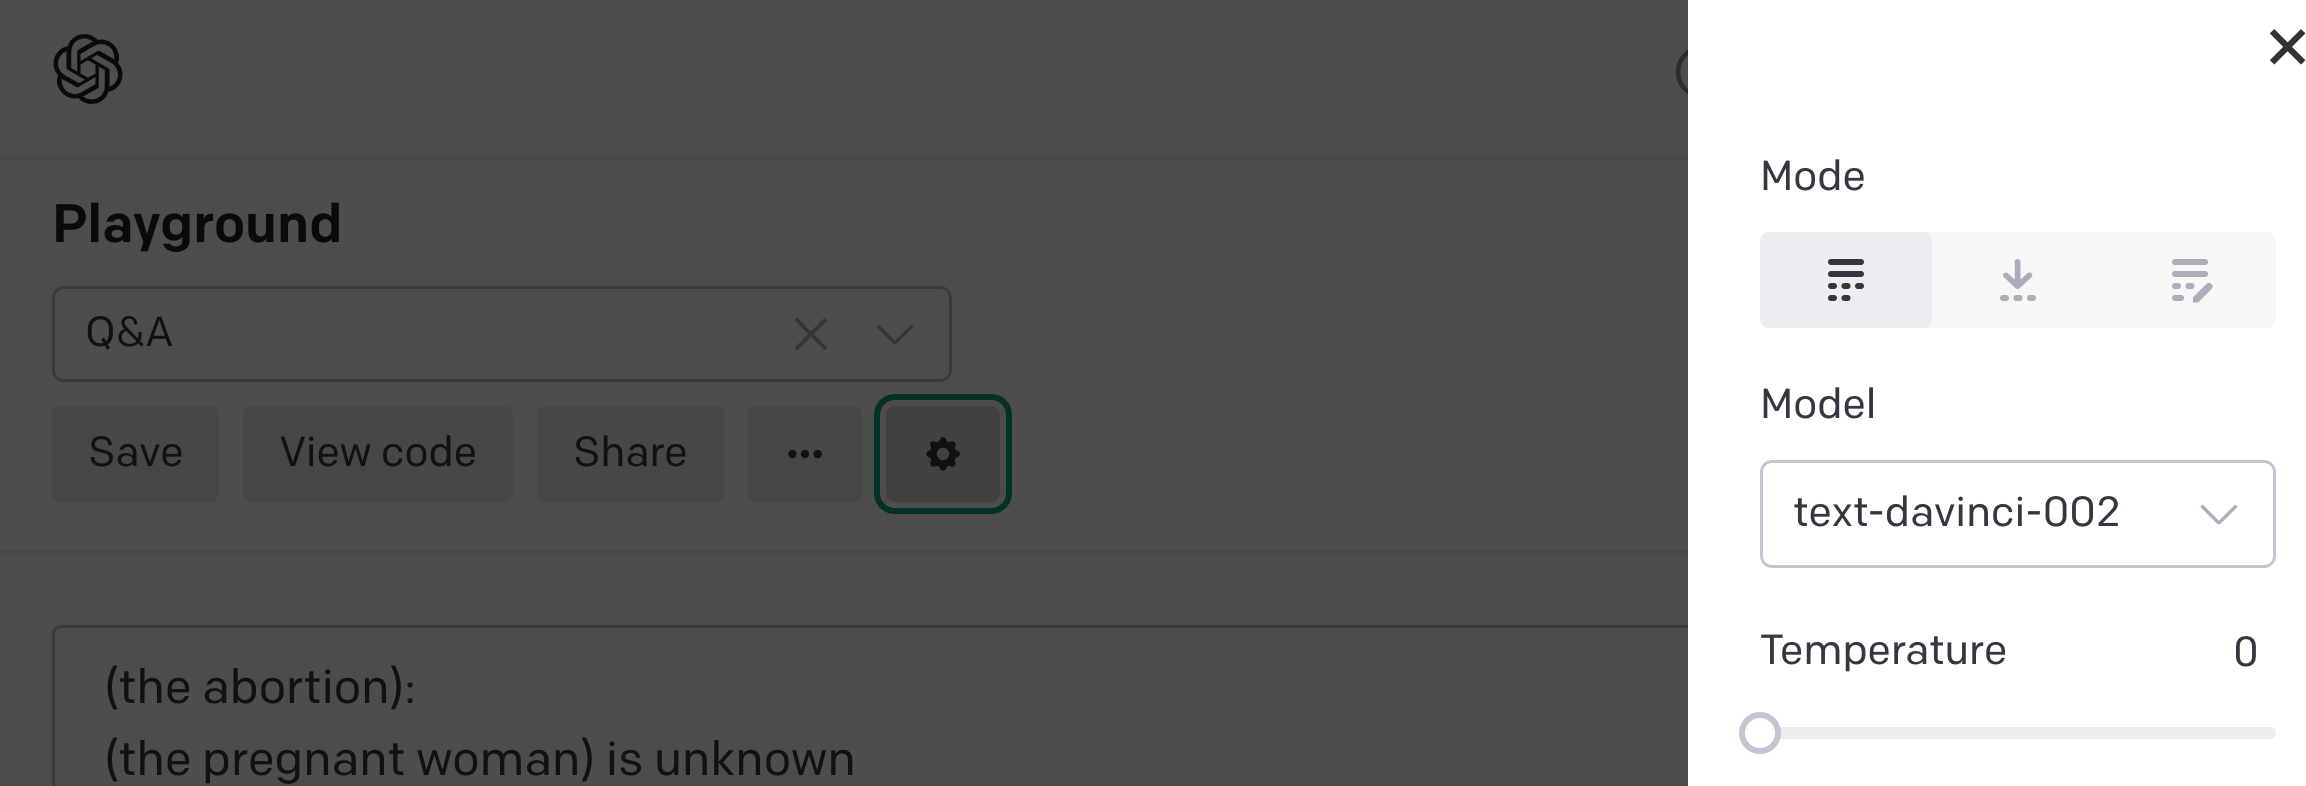
\includegraphics[width = 9in]{\images/GPT3Temperature}}

~ \hfill $\uparrow$

\slide{Temperature}

Physical temperature is a relationship between the energy and probability.

\vfill
$$P(x) = \frac{1}{Z} \;e^{\frac{-E(x)}{kT}} \;\;\;\;\;\;\;Z = \sum_x\; e^{\frac{-E(x)}{kT}}$$

\vfill
This is called the Gibbs or Boltzman distribution.

\vfill
$E(x)$ is the energy of physical microstate state $x$.


\vfill
$k$ is Boltzman's constant.

\vfill
$Z$ is called the partition function.

\slide{Temperature}

Boltzman's constant can be measured using the ideal gas law.

\begin{eqnarray*}
pV & = & NkT \\
\\
p & = & \mathrm{pressure} \\
V & = & \mathrm{volume} \\
N & = & \mbox{the number of molecules} \\
T & = & \mathrm{temperature} \\
k & = & \mbox{Boltzman's constant}
\end{eqnarray*}

\vfill
We can measure $p$, $V$, $N$ and $T$ and solve for $k$.


\slide{Temperature}

The Gibbs distribution is typically written as

$$P(x) = \frac{1}{Z}\;e^{-\beta E(x)}$$

\vfill

$\beta = \frac{1}{kT}$ is the (inverse) temperature parameter.

\vfill
``Hot'' is when $\beta$ is small and ``cold'' is when $\beta$ is large (confusing).

\slide{Temperature}

In a softmax with a temperature parameter we replace energy $E(x)$ with a score $s(x)$ and drop the negative sign.

$$\softmax_y[y] = \frac{1}{Z}\;e^{\beta s(y)}$$

\vfill
We can think of the temperature parameter $\beta$ as simply a parameter of this distribution.

\vfill
The temperature setting in GPT-3 palyground sets $\beta$ for next word selection to be $1/T$ for temperature $T$.

\slide{Temperture}

MCMC sampling typically involves a temperature parameter defining the distribution to be sampled from.

\vfill
We do not have to worry about this now, it will be discussed in detail later.

\slide{Learning Rate as Temperature}

A finite learning rate defines an equalibrium probability distribution (or density) over the model parameters.

\vfill
If we run for a long time at a large learning rate we converge to a noisy (hot) distribution with a high loss value.

\vfill
At a lower learning rate we converge to a cooler distribution with a lower loss value.

\slide{Learning Rate as Temperature}

\centerline{\includegraphics[width = 7in]{\images/annealing}}

\vfill
These Plots are from the original ResNet paper.  Left plot is for CNNs without residual skip connections, the right plot is ResNet.

\vfill
Thin lines are training error, thick lines are validation error.

\vfill
In all cases $\eta$ is reduced twice, each time by a factor of 2.

\slide{Batch Size and Temperature}

Vanilla SGD with minibatching typically uses the following update which defines the meaning of $\eta$.

\begin{eqnarray*}
\Phi_{t+1} & \;\minuseq\; & \eta \hat{g}_t \\
\\
\hat{g}_t & = & \frac{1}{B} \sum_b \hat{g}_{t,b}
\end{eqnarray*}

\vfill
Here $\hat{g}_{b}$ is average gradient over the batch.

\vfill
Under this update {\bf increasing the batch size (while holding $\eta$ fixed) reduces the temperature.}

\slide{Making Temperature Independent of $B$}

For batch size 1 with learning rate $\eta_0$ we have

\begin{eqnarray*}
\Phi_{t+1} & = &  \Phi_{t} - \eta_0\;\nabla_\Phi {\cal L}(t,\Phi_{t}) \\
\\
\Phi_{t+B} & = &  \Phi_{t} - \sum_{b=0}^{B-1} \;\eta_0\;\nabla_\Phi {\cal L}(t+b,\Phi_{\color{red} t+b-1}) \\
\\
& \approx & \Phi_t - \eta_0 \sum_b \nabla_\Phi {\cal L}(t+b,\Phi_{\color{red} t}) \\
\\
& = & \Phi_t - B\eta_0\; \hat{g}_t
\end{eqnarray*}

\vfill
For batch updates $\Phi_{t+1} = \Phi_t - B\eta_0\; \hat{g}_t$ the temperature is essentially determined by $\eta_0$ independent of $B$.

\slideplain{Making Temperature Independent of $B$}

Recent work has show that using $\eta = B\eta_0$ leads to effective learning with very large (highly parallel)
batches.

\vfill
{\bf Accurate, Large Minibatch SGD: Training ImageNet in 1 Hour}, Goyal et al., 2017.

\slide{END}

} \end{document}

